% Compile with XeLaTeX. Screenshots use demonstration accounts and data.
\documentclass[UTF8,11pt,fontset=fandol]{ctexart}
\usepackage[a4paper,left=22mm,right=22mm,top=24mm,bottom=23mm]{geometry}
\usepackage{graphicx,enumitem,caption,needspace,float}
\usepackage[hidelinks]{hyperref}
\usepackage{xurl}
\hypersetup{unicode=true,pdftitle={服务器占用可视化使用指南},
  pdfauthor={组内服务器监控项目},pdfsubject={服务器监控程序的启动、连接与资源查看}}
\ctexset{
  section={name={},number=\arabic{section},format=\Large\heiti,
    beforeskip=17pt,afterskip=9pt},
  subsection={format=\large\heiti,beforeskip=13pt,afterskip=7pt}
}
\setlength{\parindent}{2em}
\setlength{\parskip}{2pt}
\linespread{1.25}
\widowpenalty=10000
\clubpenalty=10000
\setlist[enumerate]{leftmargin=2em,itemsep=4pt,topsep=4pt,parsep=0pt}
\setlist[itemize]{leftmargin=2em,itemsep=4pt,topsep=4pt,parsep=0pt}
\renewcommand{\arraystretch}{1.25}
\newcommand{\code}[1]{{\small\texttt{\detokenize{#1}}}}
\captionsetup{font=small,labelsep=colon,skip=6pt}
\setlength{\textfloatsep}{13pt plus 3pt minus 3pt}
\setlength{\intextsep}{12pt plus 3pt minus 3pt}
\setlength{\floatsep}{10pt plus 2pt minus 2pt}
\setcounter{topnumber}{2}
\renewcommand{\topfraction}{.85}
\renewcommand{\textfraction}{.12}
\renewcommand{\floatpagefraction}{.7}
\pagestyle{plain}
\raggedbottom

\title{服务器占用可视化使用指南}
\author{}
\date{2026 年 10 月 26 日}

\begin{document}
\maketitle
\begin{abstract}
这篇指南介绍组内服务器监控程序的使用方法，包括 MacOS 和 Windows 系统下的启动、账号连接，以及 CPU、内存、磁盘和任务的查看。
程序通过 SSH 连接服务器，将各台机器的状态集中显示在本机浏览器中，方便大家在提交任务前查看资源余量，运行后查看自己的程序。
本文配合《服务器使用指南》使用，运行程序和文件传输等操作可以继续参考原指南。
\end{abstract}

\clearpage
\tableofcontents
\clearpage

\section{服务器基本信息}

组内服务器的地址和端口如下。监控程序中已经填入这些信息，使用时填写自己的账号即可。

\begin{center}
\begin{tabular}{|c|c|c|c|}
\hline
编号 & 位置 & IP 地址 & 端口 \\
\hline
1 & C814 & \code{172.17.176.141} & 88 \\
\hline
2 & 8 楼 & \code{172.17.176.242} & 22 \\
\hline
3 & 8 楼 & \code{172.17.177.147} & 22 \\
\hline
4 & C8E10 & \code{172.17.177.162} & 22 \\
\hline
5 & 6 楼 & \code{172.17.163.12} & 22 \\
\hline
6 & C8E10 & \code{172.17.177.162} & 23 \\
\hline
7 & C814 & \code{172.17.176.141} & 3 \\
\hline
\end{tabular}
\end{center}

4 号和 6 号、1 号和 7 号分别共用 IP 地址，通过不同端口连接。各台服务器的 CPU、内存和硬盘使用情况可以在监控界面中查看。

\section{监控程序的启动}
\label{sec:startup-check}

监控程序放在 \code{server_monitor.zip} 中。先完整解压压缩包，进入 \code{LabMonitor} 文件夹。
本机需要安装 Python 3.9 或更新版本，并连接校园内网或相应 VPN。

Python 的安装地址为 \url{https://www.python.org/downloads/}。

\subsection{MacOS 系统}

对于 MacOS 系统，可以通过以下步骤启动：
\begin{enumerate}
  \item 打开终端，输入 \code{python3 --version}，查看本机 Python 版本。
  \item 在解压后的文件夹中双击 \code{Start-Mac.command}。
  \item 程序启动后会自动在浏览器中打开监控界面。
\end{enumerate}

MacOS 使用系统自带的 SSH 客户端。也可以在解压后的文件夹中打开终端，输入以下命令启动：
\begin{quote}\small\ttfamily
python3 tools/launch\_monitor.py
\end{quote}
如果双击时提示文件没有执行权限，可以先在该文件夹的终端运行 \code{chmod +x Start-Mac.command}，再双击启动。

\Needspace{11\baselineskip}
\subsection{Windows 系统}

对于 Windows 系统，可以通过以下步骤启动：
\begin{enumerate}
  \item 打开命令提示符，输入 \code{python --version} 或 \code{py -3 --version}，查看本机 Python 版本。
  \item 首次使用时，双击 \code{Install-Windows.bat}。脚本会在当前文件夹创建 \code{.venv}，联网安装 SSH 连接所需的 Paramiko 及其依赖。
  \item 安装完成后，双击 \code{Start-Windows.bat} 打开监控界面。后续使用直接运行这个文件即可。
\end{enumerate}

Windows 通过 Paramiko 建立 SSH 连接。安装依赖后，也可以在当前文件夹的命令提示符运行：
\begin{quote}\small\ttfamily
.venv\textbackslash Scripts\textbackslash python.exe tools\textbackslash launch\_monitor.py
\end{quote}
Windows 版已完成 SSH 后端和凭据接口测试，完整启动流程尚待 Windows 实机验证。

\section{连接服务器}

\subsection{使用账号密码连接}

首次打开时，服务器的用户名显示为 \code{your_username}，监控处于停用状态。
没有配置免密登录的同学可以直接使用账号密码连接，步骤如下：
\begin{enumerate}
  \item 点击对应服务器右上角的齿轮，打开“编辑服务器”窗口，如图\ref{fig:connection}。
  \item 核对 IP 地址和端口，将“用户名”改为自己在这台服务器上的账号。
  \item 在“认证方式”中选择“密码”，填入登录密码。
  \item 勾选“记住用户名”和“记住密码”，后续启动时可以自动连接。
  \item 勾选“启用此服务器的监控”，点击“保存并连接”。稍等片刻，服务器状态变为“在线”后就可以查看数据。
  \item 按同样的方法设置其他服务器。不同服务器的用户名可以分别填写，暂时不用的服务器保留停用状态。
\end{enumerate}

\begin{figure}[H]
  \centering
  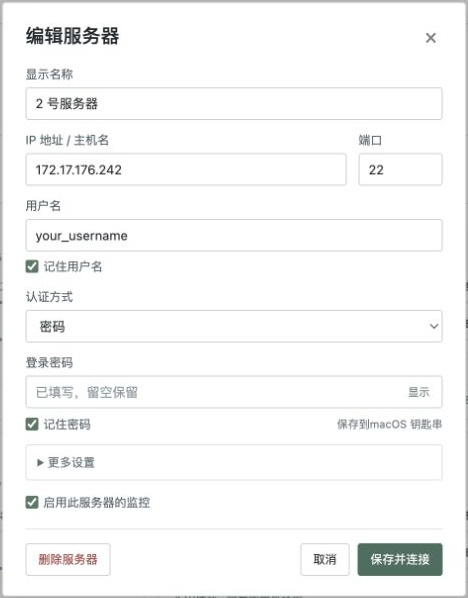
\includegraphics[width=.43\linewidth]{images/connect.jpg}
  \caption{编辑服务器连接信息，图中账号和后文数值均为演示数据}
  \label{fig:connection}
\end{figure}

“记住用户名”默认勾选。同时勾选“记住密码”后，下次启动程序会读取已保存的登录信息并连接。
密码保存在本机的 MacOS 钥匙串或 Windows 凭据管理器中。取消“记住密码”后，密码只在本次运行期间有效；取消“记住用户名”后，下次需要重新填写账号。

\subsection{免密登录与添加服务器}

已经在本机配置 SSH 密钥的同学，可以将认证方式改为“SSH 密钥”，填写本机私钥文件的路径。
更换电脑后，可以先使用密码连接，再按需要配置新电脑的免密登录。

点击界面右上角的“添加服务器”，可以填写新的 IP、端口、用户名和认证方式。
已有连接通过齿轮修改，删除连接只移除本机的监控项。

\section{资源占用与任务查看}

连接成功后，界面如图\ref{fig:overview}。上方显示在线服务器的资源汇总，下方分别列出各台服务器的 CPU、内存和进程情况。
CPU 用于执行计算，内存用于存放程序运行时的数据，磁盘用于保存代码、输入数据和结果文件。

\begin{figure}[H]
  \centering
  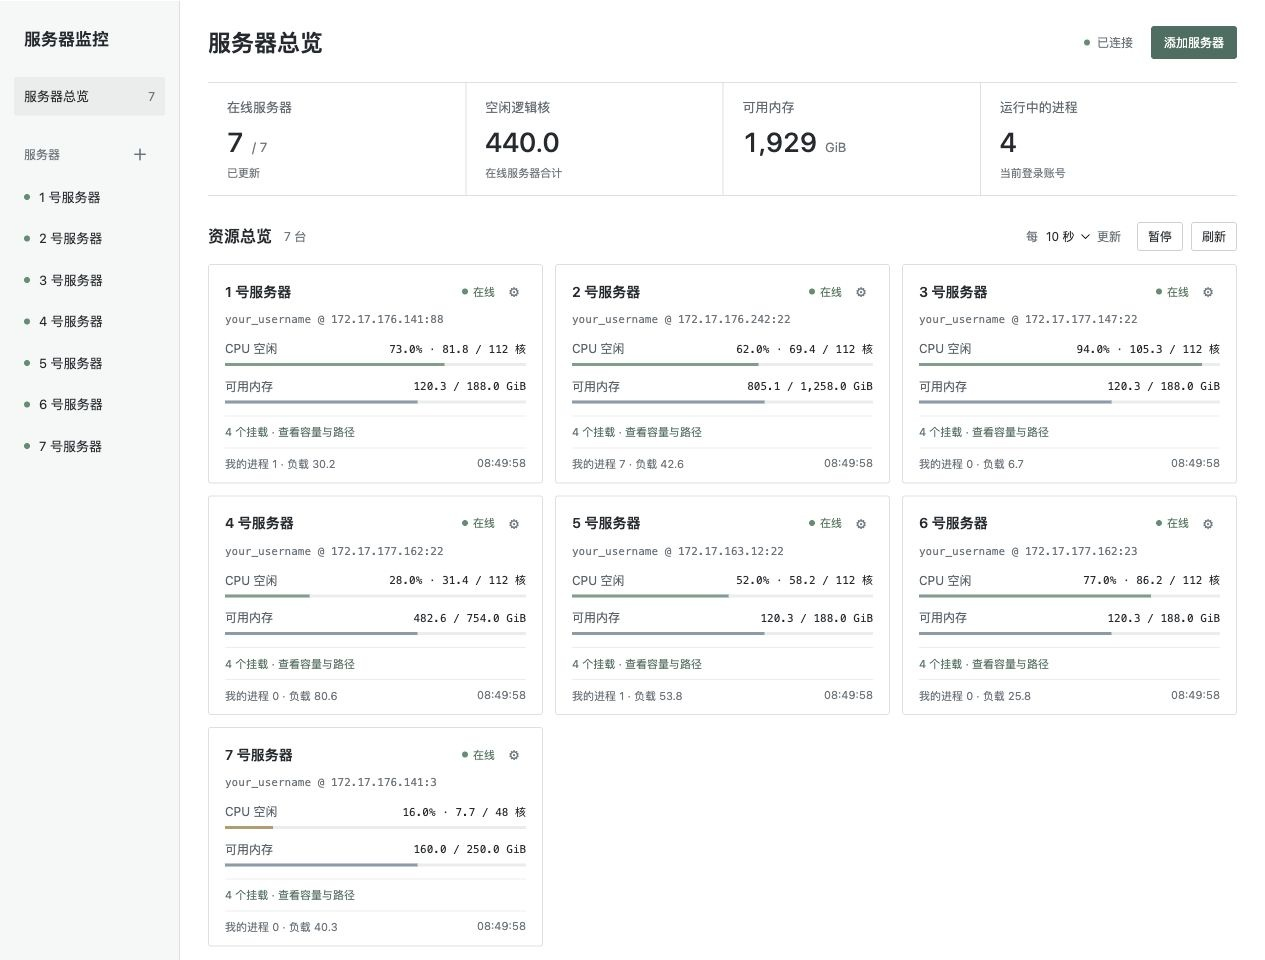
\includegraphics[width=.96\linewidth]{images/overview.jpg}
  \caption{服务器监控界面}
  \label{fig:overview}
\end{figure}

\subsection{CPU 与内存}

每台服务器的卡片中包含以下信息：
\begin{enumerate}
  \item \textbf{CPU 空闲率}：表示当前采样时间内 CPU 的空闲比例，数值越高，当前可用于计算的资源越多。
  例如图中 2 号服务器为 62\%，共 112 个逻辑核，折算约有 $112\times62\%=69.4$ 个空闲逻辑核。
  \item \textbf{可用内存}：按照“可用 / 总量”显示，单位为 GiB。
  例如 \code{805.1 / 1258.0 GiB} 表示当前约有 805.1 GiB 内存可以使用，其中包含系统可回收的缓存。
  \item \textbf{负载与更新时间}：负载是近 1 分钟内运行或等待资源的任务数量平均值，更新时间是最近一次成功采样的时间。
\end{enumerate}

CPU 空闲率和可用内存反映整台服务器的情况，上方汇总为各台在线服务器之和。

\Needspace{16\baselineskip}
\subsection{进程与任务}

向下滚动到“进程与任务”，如图\ref{fig:process}。一个正在运行的程序实例称为一个进程，一个计算任务也可能包含多个进程。

\begin{figure}[H]
  \centering
  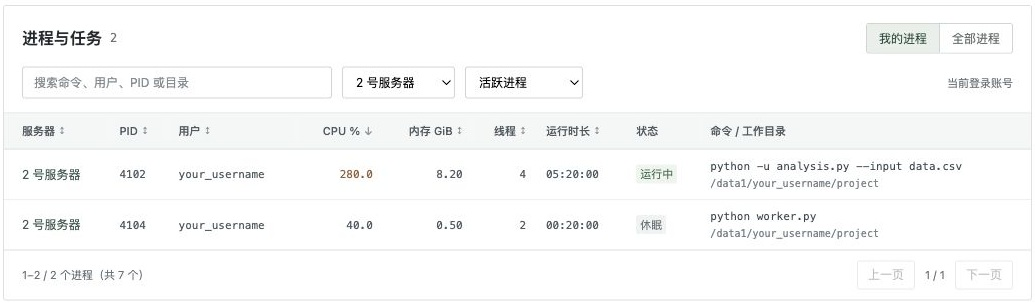
\includegraphics[width=\linewidth]{images/process.jpg}
  \caption{进程与任务列表}
  \label{fig:process}
\end{figure}

右上角可以选择两种查看方式：
\begin{itemize}
  \item \textbf{我的进程}：显示各台服务器当前登录账号下的进程。
  \item \textbf{全部进程}：显示当前账号能够查看的所有用户进程，便于了解其他同学的使用情况。
\end{itemize}

进程列表中常用字段的含义如下：
\begin{itemize}
  \item \textbf{PID、用户}：PID 是进程在该服务器上的编号，用户是运行这个进程的账号。
  \item \textbf{CPU \%}：100\% 对应一个逻辑核。图中的 280\% 约使用 2.8 个逻辑核，多线程程序可以超过 100\%。
  \item \textbf{内存 GiB}：该进程当前驻留内存（RSS）。共享内存可能同时计入多个进程。
  \item \textbf{线程、运行时长、状态}：分别表示进程的线程数、已运行时间和当前状态。“休眠”通常表示在等待数据、I/O 或其他任务。
  \item \textbf{命令 / 工作目录}：显示启动程序的命令，以及程序所在的目录。点击进程所在行可以查看完整内容。
\end{itemize}

上方“运行中的进程”统计状态为 R 或采样期间有 CPU 占用的进程。进程列表默认只显示这些活跃进程；短暂休眠但采样期间仍有计算的进程也会保留。
状态下拉框可选择全部状态、运行中、休眠、I/O 等待、已停止或僵尸进程。
搜索框可以按程序名、用户名、PID 或工作目录筛选，点击列名可以排序。状态筛选会在排序和自动更新时保留。
点击某台服务器或使用下拉框，可以只看该台机器；点击左侧“服务器总览”恢复查看所有服务器。

\subsection{磁盘容量与挂载路径}

点击服务器卡片上的“查看容量与路径”，可以跳到该服务器的“磁盘与挂载”列表，如图\ref{fig:disk}。
每一行显示一个存储挂载点的总容量、已用容量、可用容量和挂载路径，容量单位为 GiB（$1\,\mathrm{GiB}=2^{30}$ 字节）。

\begin{figure}[H]
  \centering
  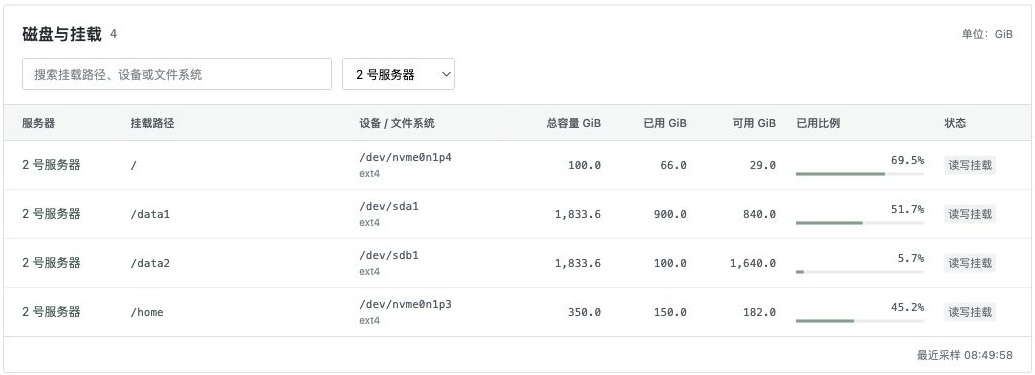
\includegraphics[width=\linewidth]{images/disks.jpg}
  \caption{磁盘容量与挂载路径}
  \label{fig:disk}
\end{figure}

挂载路径是存储设备在服务器目录中的入口。例如 \code{/data1} 是一个挂载路径，保存在 \path{/data1/your_username/project} 中的文件通常使用这一行所显示的磁盘空间。

查看磁盘时主要关注以下内容：
\begin{enumerate}
  \item \textbf{挂载路径}：各台服务器可能使用 \code{/data}、\code{/data1} 或 \code{/mnt/...} 等路径，实际路径可以从界面复制。
  保存较大的文件时，在数据盘中使用自己账号的目录。
  \item \textbf{可用容量}：表示文件系统的剩余可用空间。例如预计保存 50 GiB 的结果，可以选择可用容量充足的目录，并考虑中间文件和日志的大小。
  \item \textbf{设备 / 文件系统}：如 \code{/dev/sda1} 和 \code{ext4}，分别表示设备名称和文件系统类型。
  \item \textbf{挂载状态}：“读写挂载”表示该文件系统以读写方式挂载，具体文件夹的写权限由账号权限决定。
\end{enumerate}

部分文件系统会预留空间，因此“已用 + 可用”可能小于“总容量”。界面已用比例按“已用 $\div$（已用 + 可用）”计算。
同一文件系统可能出现在多个挂载路径，容量按对应文件系统计算。

\section{日常使用}

界面默认每 10 秒更新一次，可以选择 5、10、30 或 60 秒，也可以点击“刷新”立即采样。
新数据会替换原来的内容，搜索条件和表格位置会保留。连接中断时，界面会显示错误和最近一次成功采样的数据。

提交任务之前，建议查看 CPU 空闲量、可用内存和目标目录的磁盘余量，再根据程序需求设置线程数和任务数量。
例如一个任务预计使用 8 个线程、峰值内存 12 GiB、输出 50 GiB，就选择这三项资源均有余量的服务器，并按照原《服务器使用指南》中的方法登录和运行。
运行后可以在“我的进程”中查找程序名、PID 和工作目录，结合输出日志查看计算进度和结果。

“暂停”用于停止后续采样，“退出程序”用于关闭本机监控服务。
只关闭浏览器标签页时，服务仍在本机运行，重新双击启动文件可以打开原界面。
退出监控不会影响服务器上正在运行的任务。

\Needspace{9\baselineskip}
\section{常见问题}

\begin{enumerate}
  \item \textbf{启动时提示缺少 Python 或 Paramiko。}
  先按第\ref{sec:startup-check}节的方法检查 Python 版本；Windows 首次使用时运行 \code{Install-Windows.bat}。
  安装依赖失败时，检查本机互联网连接后重新运行安装脚本。
  \item \textbf{连接超时。}
  检查校园内网或 VPN、IP 地址和端口。单台服务器无法连接时，可以向相应管理员确认机器状态。
  \item \textbf{出现 \code{Permission denied}。}
  核对该服务器的用户名和密码，认证方式选择“密码”。修改后点击“保存并连接”或“刷新”重试。
  \item \textbf{重启程序后需要重新登录。}
  在连接设置中勾选“记住用户名”和“记住密码”，重新保存一次。未勾选“记住密码”时，下次启动需要重新填写密码。
  \item \textbf{远端找不到 Python。}
  在连接的“更多设置”中填写服务器上的 Python 解释器路径。
  7 号服务器已预设为 \code{/usr/local/anaconda3/bin/python3}。
  \item \textbf{进程列表没有显示预期程序。}
  检查服务器、登录账号、状态筛选和搜索条件，也可以选择“全部状态”查看；程序已经退出时，可以到任务目录查看日志和结果。
  \item \textbf{浏览器无法连接监控页面。}
  重新双击启动文件，使用程序自动打开的地址。浏览器中的 \code{127.0.0.1} 是本机地址，端口由程序自动选择。
  \item \textbf{提示服务器主机密钥变化。}
  向管理员确认服务器是否重装或更换，再更新本机的连接记录。
\end{enumerate}

\section{参考资料}

本文参考刘雷轶男、智朝晖编写的《服务器使用指南》（2024 年 12 月 30 日），原文件保存在项目的 \code{docs/references/} 中。
监控界面和连接方式按本程序当前版本说明，服务器容量以实际采样结果为准。

程序启动文件和说明书位于分发包的主目录。TeX 源码及插图保存在项目的 \code{docs/guide/} 中。

\end{document}
